\section{The need for high-level abstractions}
We start the discussion of programming for parallel systems and in particular for \GPU systems by looking thoroughly at an application example.
By doing so we will identify challenges opposed upon application developers which arise from typical features of parallel hardware architectures.
We will then derive from these challenges requirements to a potential high-level programming model.


% ============================================================================ %
\subsection{Challenges of \GPU programming}
\label{section:opencl-example}
We choose to investigate a real-world application rather than a simple benchmark, in order to identify not only fundamental challenges every application developer targeting \GPU systems faces, but also practical programming challenges which become only visible for more complex applications, \eg, managing the execution of multiple compute kernels.

Our example application is the LM OSEM algorithm~\cite{ReaderErFlOt1998, SchellmannGoMeKoScWuBu2009} for image reconstruction used in Positron Emission Tomography (PET).
In PET, a radioactive substance is injected into a human or animal body, which is then placed inside a PET scanner that contains several arrays of detectors.
As the particles of the applied substance decay, positrons are emitted (hence the name PET) and annihilate with nearby electrons, such that two photons are emitted in the opposite directions (see \autoref{fig:scanner and detector}).
These ``decay events'' are registered by two opposite detectors of the scanner which records these events.
Data collected by the PET scanner are then processed by a reconstruction algorithm to obtain a resulting image.

\begin{figure}
  \centering
  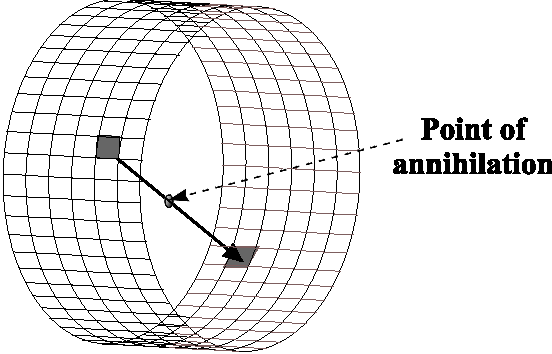
\includegraphics[scale=0.50]{ICCS/ringscanner}
  \caption{Two detectors register an event in a PET-scanner}
  \label{fig:scanner and detector}
\end{figure}

\subsubsection{The LM OSEM Algorithm}
List-Mode Ordered Subset Expectation Maximization \cite{ReaderErFlOt1998} (called LM OSEM in the sequel) is a block-iterative algorithm for 3D image reconstruction.
LM OSEM takes a set of events from a PET scanner and splits them into $s$ equally sized subsets.
Then, for each subset $S_l, l \in {0, \ldots, s-1}$, the following computation is performed:
\begin{equation}
  f_{l+1}=f_{l}c_{l};\quad c_{l}=\dfrac{1}{A_N^T \textbf{1}} \sum_{i \in S_{l}} (A_i)^T \dfrac{1}{A_{i} f_{l}}.
\label{equ:lm_osem}
\end{equation}

Here $f \in \mathbb{R}^n$ is a 3D image in vector form with dimensions $n = (X \times Y \times Z)$, $A$ it the so-called system matrix, element $a_{ik}$ of row $A_i$ is the length of intersection of the line between the two detectors of event $i$ with voxel $k$ of the reconstruction image, computed with Siddon's algorithm \cite{Siddon1985}.
$\rfrac{1}{A_N^T \textbf{1}}$ is the so-called normalization vector; since it can be precomputed, we will omit it in the following.
The multiplication $f_{l}c_{l}$ is performed element-wise.
Each subset's computation takes its predecessor's output image as input and produces a new, more precise image.

The structure of a sequential LM OSEM implementation is shown in \autoref{lst:lmosem:seq_code}.
The outermost loop iterates over the subsets.
The first inner loop (step 1, lines~\autoref{lst:lmosem:seq_code:step1:begin}--\autoref{lst:lmosem:seq_code:step1:end}) iterates over subset's events to compute $c_l$, which requires three sub-steps:
row $A_i$ is computed from the current event using Siddon's algorithm;
the local error for row $A_i$ is computed and, finally, added to $c_l$.
The second inner loop (step 2, lines~\autoref{lst:lmosem:seq_code:step2:begin}--\autoref{lst:lmosem:seq_code:step2:end}) iterates over all elements of $f_l$ and $c_l$ to compute $f_{l+1}$.
\begin{figure}
\begin{lstlisting}[
  caption={Sequential code for LM OSEM comprises one outer loop with two nested inner loops.},
  label={lst:lmosem:seq_code}]
for (int l = 0; l < subsets; l++) {
  // read subset

  // step 1: compute error image $c_l$
  for (int i = 0; i < subset_size; i++) { $\label{lst:lmosem:seq_code:step1:begin}$
    // compute $A_i$
    // compute local error
    // add local error to $c_l$
  } $\label{lst:lmosem:seq_code:step1:end}$

  // step 2: update image estimate $f$
  for (int k = 0 ; k < image_size; k++) { $\label{lst:lmosem:seq_code:step2:begin}$
    if (c_l[k] > 0.0) { f[k] = f[k] * c_l[k]; }
  } $\label{lst:lmosem:seq_code:step2:end}$
}
\end{lstlisting}
\end{figure}

\subsubsection{Parallelization of LM OSEM in OpenCL}
\label{sec:parallel_implementation}
LM OSEM is a rather time-consuming algorithm that needs parallelization:
a typical 3D image reconstruction processing $6 \cdot 10^7$ input events for a $150 \times 150 \times 280$ voxel PET image takes more than two hours on a modern PC.

Although the iterations of the outer loop in \autoref{lst:lmosem:seq_code} are inherently sequential, we can parallelize the two calculation steps within one iteration as shown in \autoref{fig:lmosem:em_distribution} for a system comprising one CPU and two GPUs.
Note that these steps require different data distribution patterns:
\begin{itemize}
  \item[] \emph{Step 1:} Subset's events are copied from the CPU to all GPUs (\emph{upload}) to compute the summation parts of $c_l$ concurrently. This step requires that the complete image estimate $f_l$ is available on all GPUs.
  \item[] \emph{Step 2:} For computing the next image estimate $f_{l+1}$ in parallel, the current image estimate $f_l$ and the error image $c_l$ computed in step 1 have to be distributed in disjoint parts (blocks) among all GPUs.
\end{itemize}

\begin{figure}
  \centering
  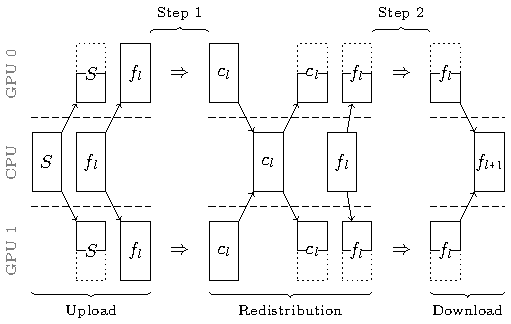
\includegraphics[width=0.6\textwidth]{ICCS/em_distribution}
  \caption{Parallelization schema of the LM OSEM algorithm.}
  \label{fig:lmosem:em_distribution}
\end{figure}
Thus, the parallelization schema in \autoref{fig:lmosem:em_distribution} requires a \emph{data redistribution} phase between the two computation steps.
During step 1, each GPU computes a partial sum of $c_l$ which are then summed up and redistributed disjoinlty to all GPUs after step 1.
Note that for step 1, each GPU requires a full copy of the image estimate, while in step 2 all GPUs update disjoint parts of it.
After step 2, the disjoint parts of the image estimate are copied from all GPUs back to the CPU (\emph{download}).

\bigskip\noindent
In the following, we describe how the phases in the parallelization schema in \autoref{fig:lmosem:em_distribution} are implemented using OpenCL.

\paragraph{Upload}
\autoref{lst:lmosem:upload} shows the simplified OpenCL implementation of the upload phase.
Uploading of the event vector $S$ is performed in lines \autoref{lst:lmosem:upload:1:start}--\autoref{lst:lmosem:upload:1:end}, while lines \autoref{lst:lmosem:upload:2:start}--\autoref{lst:lmosem:upload:2:end} upload the image estimate $f_l$.
In OpenCL, we have to manage each GPU explicitly, therefore, for each GPU, we create an array of buffers (\texttt{s\_gpu} in line~\autoref{lst:lmosem:upload:1:cl_false} and \texttt{f\_gpu} in line~\autoref{lst:lmosem:upload:2:cl_false}) and we use a loop (line \autoref{lst:lmosem:upload:loop}) to repeat all memory operations for each GPU.
For performance reasons, we use asynchronous copy operations, specified using the \texttt{CL\_FALSE} flag (lines \autoref{lst:lmosem:upload:1:cl_false} and \autoref{lst:lmosem:upload:2:cl_false}): this allows data transfers to multiple GPUs to overlap.
We perform different operations with $S$ (distribute among all GPUs) and $f_l$ (copy to each GPU), therefore, there are differences when specifying the amount of bytes to copy (lines \autoref{lst:lmosem:upload:1:amount} and \autoref{lst:lmosem:upload:2:amount}) and the offsets in the CPU memory (lines \autoref{lst:lmosem:upload:1:offset} and \autoref{lst:lmosem:upload:2:offset}).
Altogether eleven such memory operations -- each with different amounts of bytes and offsets -- appear in the OpenCL source code.

\begin{lstlisting}[float,
  caption={Implementation of the upload phase in OpenCL (omitting error checks for brevity)},
  label={lst:lmosem:upload}]
for (int gpu = 0; gpu < gpu_count; gpu++) {$\label{lst:lmosem:upload:loop}$
  // upload $S$
  clEnqueueWriteBuffer( command_queue[gpu], $\label{lst:lmosem:upload:1:start}$
        s_gpu[gpu], CL_FALSE, 0,$\label{lst:lmosem:upload:1:cl_false}$
        sizeof(float) * size_of_s / gpu_count,$\label{lst:lmosem:upload:1:amount}$
        (void*)&s_cpu[ gpu * size_of_s / gpu_count ],$\label{lst:lmosem:upload:1:offset}$
        0, NULL, NULL );$\label{lst:lmosem:upload:1:end}$

  // upload $f_l$
  clEnqueueWriteBuffer( command_queue[gpu], $\label{lst:lmosem:upload:2:start}$
        f_gpu[gpu], CL_FALSE, 0,$\label{lst:lmosem:upload:2:cl_false}$
        sizeof(float) * size_of_f,$\label{lst:lmosem:upload:2:amount}$
        (void*)&f_cpu[0],$\label{lst:lmosem:upload:2:offset}$
        0, NULL, NULL );$\label{lst:lmosem:upload:2:end}$
}
\end{lstlisting}

\paragraph{Step 1}
The implementation of step 1 performs the operations shown in \autoref{lst:lmosem:seq_code}.
Because of GPU memory restrictions, the OpenCL implementation is not straightforward, therefore, we will not show the detailed code here.
An OpenCL kernel is launched where each work item processes multiple events one after another.
For each event first $A_i$ is computed, then the local error for $A_i$ is computed using the current image estimate $f_l$ which is finally added to $c_l$.

In \autoref{equ:lm_osem} $A_i$ represents the \emph{path} of a detected line through the 3D image space.
In mathematics it is convenient to think of this as a sparse vector containing the length of the intersection of the line with a given voxel in the image space.
As most voxels are not intersected by the line, most entries in the vector remain zero.
Therefore, in the OpenCL code $A_i$ is represented as an array of pairs, where the first entry of each pair is the index of a voxel in the image space and the second entry is the length of the intersection with this voxel.

Synchronization between work items in OpenCL is highly restricted, \ie, synchronization is only possible for work items organized in the same work group.
Therefore, it is not possible to efficiently protect the writing operation to $c_l$ to avoid race conditions.
We have conducted studies and found that for this particular algorithm these race conditions are acceptable as they do not substantially decrease the numerical accuracy of the computed result~\cite{SchellmannGoMeKoScWuBu2009}.


\paragraph{Redistribution}

\begin{lstlisting}[float,
  caption={OpenCL pseudocode for the redistribution phase},
  label={lst:lmosem:redistribution}]
// download all c_l values from the GPUs to the CPU
cl_event events[gpu_count];
for (int gpu = 0; gpu < gpu_count; gpu++) {
  clEnqueueReadBuffer( ..., &events[gpu] );$\label{lst:lmosem:redistribution:operation}$
}
clWaitForEvents(gpu_count, events);$\label{lst:lmosem:redistribution:wait}$

// combine data on CPU
combine( ... );$\label{lst:lmosem:redistribution:combine}$

// upload block of the new c_l version to each GPU
for (int gpu = 0; gpu < gpu_count; gpu++) {
  clEnqueueWriteBuffer( ... );
}
\end{lstlisting}

\autoref{lst:lmosem:redistribution} shows an OpenCL pseudocode for the redistribution phase.
To download the data from all GPUs, we use the \texttt{clEnqueueReadBuffer} function and perform the operations asynchronously, but this time, we have to wait for the operations to finish.
For such synchronization, OpenCL uses \emph{events}, associated with an operation (line \autoref{lst:lmosem:redistribution:operation}) for waiting for the operation to finish (line \autoref{lst:lmosem:redistribution:wait}).
After all downloads have finished, we combine the different values of $c_l$ to a new value of $c_l$ on the CPU (line \autoref{lst:lmosem:redistribution:combine}), and upload the blocks of $c_l$ to the GPUs.
Even if we only copied data between GPUs, without processing them on the CPU, we still would have to download them to the CPU because direct GPU-to-GPU transfers are currently not possible in OpenCL.

\paragraph{Step 2}
\autoref{lst:lmosem:step_2} shows the implementation of step 2.
In OpenCL, computations are specified as \emph{kernels} which are created from the source code specifying the computation.
The computation in step 2 is, therefore, described as a string in lines \autoref{lst:lmosem:step_2:string:start}--\autoref{lst:lmosem:step_2:string:stop}.
The operations used here are the same as in the sequential code.

For executing the computations of step 2, we have to perform the following steps for each GPU:
\begin{itemize}
  \item create an OpenCL kernel from the source code (requires 50 lines of code in OpenCL);
  \item compile the kernel specifically for the GPU (requires 13 lines of code in OpenCL);
  \item specify kernel arguments one-by-one using the \texttt{clSetKernelArg} function (line \autoref{lst:lmosem:step_2:args:start} -- \autoref{lst:lmosem:step_2:args:stop});
  \item specify execution environment, i.\,e., how many instances of the kernel to start (line \autoref{lst:lmosem:step_2:env:start} -- \autoref{lst:lmosem:step_2:env:stop});
  \item launch the kernel (line \autoref{lst:lmosem:step_2:kernel:start} -- \autoref{lst:lmosem:step_2:kernel:stop}).
\end{itemize}
\begin{lstlisting}[float,
  caption={Implementation of step 2 in OpenCL (omitting error checks for brevity)},
  label={lst:lmosem:step_2}]
// step 2 (in $\autoref{fig:lmosem:em_distribution}$)
source_code_step_2 =
  "kernel void step2(global float* f, global float* c_l,$\label{lst:lmosem:step_2:string:start}$
                     int offset, int size) {
    int id = get_global_id(0) + offset;
    if (id < size && c_l[id] > 0.0){ f[id] = f[id]*c_l[id];}$\label{lst:lmosem:step_2:zip}$
   }";$\label{lst:lmosem:step_2:string:stop}$

for (int gpu = 0; gpu < gpu_count; gpu++) {
  // create kernel (50 lines of code)
  // compile kernel (13 lines of code)

  // specifying kernel arguments:
  clSetKernelArg(kernel_step2[gpu], 0, sizeof(cl_mem),$\label{lst:lmosem:step_2:args:start}$
                 (void*)&f_buffer[gpu]);
  clSetKernelArg(kernel_step2[gpu], 1, sizeof(cl_mem),
                 (void*)&c_l_buffer[gpu]);
  int offset = gpu * (size_of_f / gpu_count);
  clSetKernelArg(kernel_step2[gpu], 2, sizeof(int),
                 (void*)&offset);
  int size   = MIN( (gpu + 1) * (size_of_f / gpu_count),
                    size_of_f );
  clSetKernelArg(kernel_step2[gpu], 3, sizeof(int),
                 (void*)&size);$\label{lst:lmosem:step_2:args:stop}$

  // specify execution environment
  int local_work_size[1]  = { 32 };$\label{lst:lmosem:step_2:env:start}$
  int global_work_size[1] =
        { roundUp(32, size_of_f / gpu_count) };$\label{lst:lmosem:step_2:env:stop}$
  // launch the kernel
  clEnqueueNDRangeKernel($\label{lst:lmosem:step_2:kernel:start}$
        command_queue[gpu], kernel_step2[gpu],
        1, NULL, &global_work_size, &local_work_size, 0,
        NULL, NULL); }$\label{lst:lmosem:step_2:kernel:stop}$
\end{lstlisting}


\paragraph{Download}
The implementation of the download phase is similar to the upload phase as shown in \autoref{lst:lmosem:upload}.


% ============================================================================ %
\subsection{Requirements to a High-Level Programming Model}
\label{section:requirements}
The described implementation of the example application reveals the main problems and challenges that application developers have to overcome when targeting \GPU systems.
Our analysis show that to simplify programming for a system with multiple \GPUs, at least the following three high-level abstraction are desirable:

\paragraph{Parallel container data types}
Compute-intensive applications typically operate on a (possibly big) set of data items.
As shown in \autoref{lst:lmosem:upload}, managing memory is error-prone because low-level details, like offset calculations, have to be programmed manually.

A high-level programming model should be able to make collections of data automatically accessible to all processors in a system and it should provide an easy-to-use interface for the application developer.

\paragraph{Recurring patterns of parallelism}
While each application performs (of course) different concrete operations, the general structure of parallelization often resembles parallel patterns that are commonly used in many applications.
In step~1, for computing the error image~$c_l$, the same sequence of operations is performed for every event from the input subset, which is the well-known \emph{map} pattern of data-parallel programming~\cite{GorlatchCo2011}.
In step~2, two images (the current image estimate~$f_l$ and the error image~$c_l$) are combined element-wise into the output image~($f_{l+1}$), see line~\autoref{lst:lmosem:step_2:zip} of \autoref{lst:lmosem:step_2}, which is again a well-known pattern of parallelism commonly called \emph{zip}.

It would be, therefore, desirable to express the high-level structure of an application using pre-defined common patterns, rather than describing the parallelism manually in much detail.

\paragraph{Distribution and redistribution mechanisms}
To achieve scalability of applications on systems comprising multiple \GPUs, it is crucial to decide how the application's data are distributed across all available \GPUs.
Distributing and re-distributing data in \OpenCL is cumbersome because data transfers have to be managed manually and performed via the \CPU, as shown in \autoref{lst:lmosem:upload} and \autoref{lst:lmosem:redistribution}.

Therefore, it is important for a high-level programming model to allow both for describing the data distribution and for changing the distribution at runtime.
